\documentclass[ncrna,article,submit,moreauthors,pdftex,10pt,a4paper]{mdpi}

\usepackage{color}
\usepackage[utf8]{inputenc}

\Title{Supplementary File 1}
\Author{}
\address{}

\begin{document}
\section{Gene structure analysis}

Fig. \ref{comparison} shows the distribution of introns per gene between the dataset and GENCODE v19. We compared the number of introns of every gene from the dataset as we calculated with the same genes as found in GENCODE. Although a similarity could be noticed, we computed a number of genes to have higher number of introns than in GENCODE.
%\clearpage
\begin{figure}[H]
 \centering
 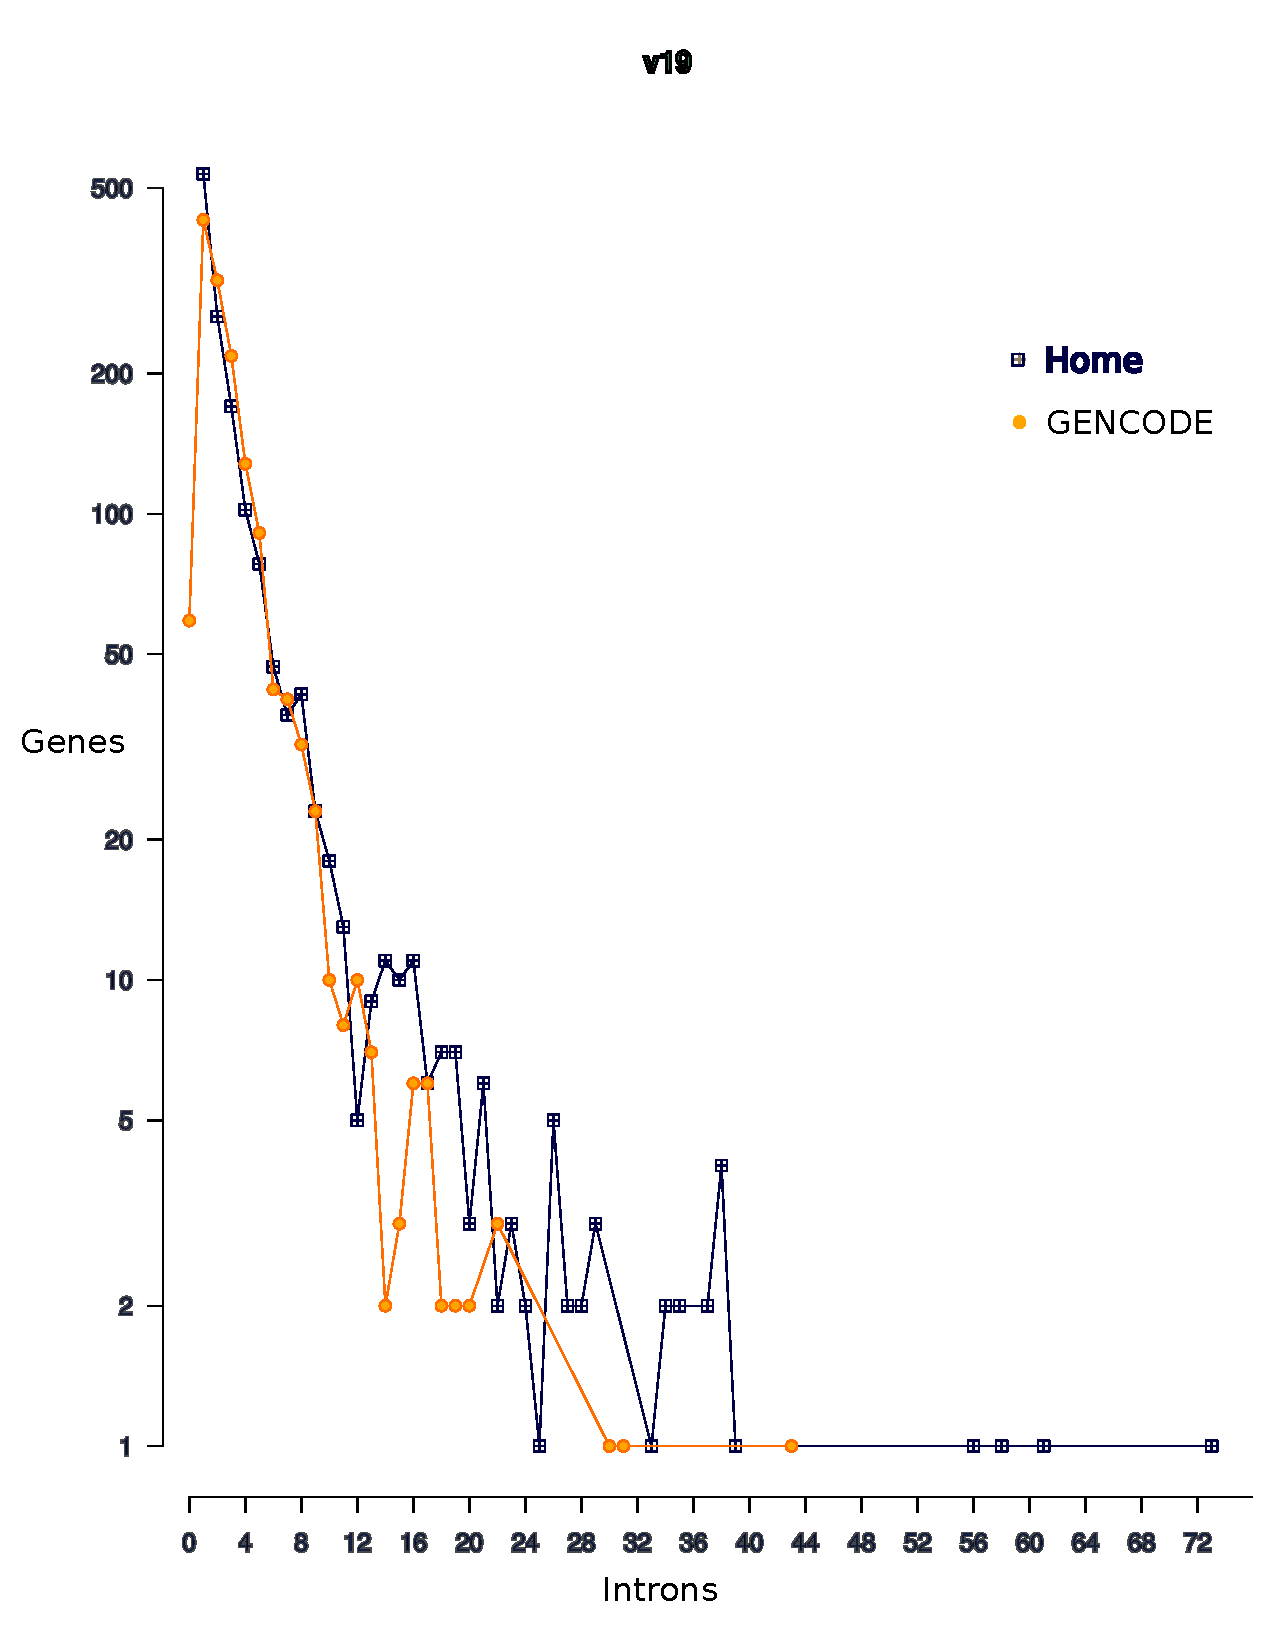
\includegraphics[height = 12 cm, width=14 cm]{comparison_plot_2}
 \caption{The annotations of the lincRNAs from the RNA-Seq data were compared against the annotations of the same lincRNAs found in GENCODE. A considerable number of genes having more introns than reported in GENCODE is shown here.}
 \label{comparison}
\end{figure}

Our dataset comprises of 5,257 long intergenic noncoding RNAs (lincRNAs). 3,926 genes were found to be present in GENCODE v7 \cite{harrow2012}. We have analysed the individual transcripts against the GENCODE v7 dataset and found that 4,563 of them were reported as opposed to 8154 GENCODE transcripts. We have also found that mean of exons is 2 for our dataset.

GENCODE v24 reports 15,941 lncRNA genes, among them 7,674 are lincRNAs. We calculated the number of genes from our dataset are present in GENCODE v24, which is 4,961. 7,487 transcripts were found against 12,656 lincRNA transcripts with a mean of slightly above 2 exons.

\bibliographystyle{mdpi}
\bibliography{references}

\end{document}
